\chapter{Light Clients}\label{chapter.light}

So far, all the participants in our network have been downloading the whole blockchain,
including all transactions, and rebuilding the transaction graph to verify that everything
is well. This includes both miners, as well as wallets, who need to have access to a node.
A node that performs this whole verification is known as a \emph{full node}\index{Full Node}.

As the blockchain contains all transactions ever made by anyone, this can be quite inefficient
if the purpose is to just operate a wallet. After all,
why does a wallet, which concerns itself about only very specific and limited public keys,
need to know about everyone's transactions? It is only interested in transactions that concern
the public keys it holds, as well as verifying that any incoming money is truly existent and
not forged.

As time goes by and the blockchain grows, this problem becomes more pronounced, because transactions
are only ever added but never removed. The larger the running time of the system, the more data
that has to be downloaded by a node, and the more time this takes.
This is especially bothersome for a node that holds only the genesis
block and is booting into the system for the first time. This problem is known as the
\emph{bootstrapping problem}\index{Bootstrapping Problem}.
From a practical standpoint, a blockchain system is unusable if a mobile wallet app takes
a few days to synchronize with the rest of the network when first installed, and in the meantime
uses all of the user's bandwidth to download this data and a significant amount of battery
for signature validation.

Of course, a mobile app could use a custodian wallet that holds its private keys, or
utilize a trusted node while holding its own private key locally. However, this entails
a level of centralization that we would like to avoid.

Towards this end, we will modify our blockchain system to allow a node to
synchronize quickly. Our nodes will only download transactions that are of interest
to them, as well as the proof-of-work of the chain, but no transactions that do not
concern them.
These nodes are known as \emph{light nodes}\index{Light Node}, and the protocol
we will develop is called \emph{simple payment verification}\index{Simple Payment Verification} (SPV).

{\color{red}
\begin{itemize}
\item The Random Oracle model
\item Random Oracles are collision resistant
\item Random Oracle collision resistance security proof
\item Random Oracles are pre-image resistant
\item Random Oracle pre-image resistance security proof
\item Block predictions are difficult in the Random Oracle model
\item Authenticated data structures
\item Merkle trees
\item Building a complete Merkle tree from data
\item Building a Merkle tree proof
\item Validating a Merkle tree proof
\item Merkle trees in the torrent protocol
\item Merkle tree game-based security definition
\item Merkle tree security theorem and proof
\item The SPV protocol
\item Light clients
\item Sparse Merkle trees, Merkle-Patricia tries: Polynomial data in an exponential sea
\item Light mining using block state commitments
\item State commitment in block headers
\end{itemize}
}

\section{Light Clients}

How to run a blockchain node efficiently? Efficiency has multiple dimensions: storage, communication, and computation. For most application scenarios, the blockchain node has limited resources. For example, if we store all the data of the chain, it would take gigabytes of storage. Validating every transaction in the network would be very heavy work for a phone. Therefore, a light client is needed for these resource-limited nodes.

\subsection{Storage Efficiency: Merkle Trees}

For a light client, it is better to save the data at a server and retrieve data at usage. However, we need to prove the integrity of the retrieved data. Hash functions are useful in this case. Suppose that we wanted to store a file on a server and verify that we receive the correct file from the server. We could hash the file and store the hash (checksum) locally. When we request files from the data server, we validate the checksum of the retrieved file to verify that it is the exact file we saved on the server. However, this requires clients to retrieve the entire file to validate its integrity even if only a 1 kilobyte chunk is needed.

We can also split the file into chunks and hash each chunk. This reduces the communication complexity: clients only need the chunk to be transferred. However, this requires more hash key storage for the client. The client needs to store one hash per chunk, making the storage complexity linear in the size of the file. There is a trade off between communication complexity and storage complexity: with large chunks, comes high communication complexity and with small chunks, comes high storage complexity.

Our goal is to achieve low storage and low communication. Specifically, storage with $O(1)$ complexity and communication with $O(\log n)$ complexity where $n$ is the number of chunks of the file. And this is done with a data structure called Merkle tree.

\subsection{Data Structure: Merkle Tree}

Files are split into $n$ data chunks.
$$
D: D[0], D[1], ..., D[n-1]
$$

A binary tree of depth $\mu$ is created, where there are $2^\mu = n$ leaves (for simplicity, assume that $n$ is a power of 2). Each node in the binary tree stores a hash $h$ which is the hash of its children concatenated.
$$
h \coloneqq H(h[\mathrm{left}] \mathbin\Vert h[\mathrm{right}])
$$

Nodes on the leaves store the hash of the corresponding data chunk. The client stores the Merkle tree root (MTR) $h_\epsilon$. When a data chunk is requested, the server sends the data chunk, along with every sibling hash value to the clients as shown in Figure \ref{fig.merkleTree}. For example, when data chunk at index $j$ is requested, the server sends $D[j]$, $\pi_0$, $\pi_1$, $\pi_2$, and $\pi_3$ to the client. The client walks from the received data chunk all the way up to the root to check if the hash values are intact. From calculating $e_0$ by hashing the data chunk, to the top level $e_{\mu+1}$, the client calculates $e_k = H(e_{k-1} \mathbin\Vert \pi_{k-1})$ or $e_k = H(\pi_{k-1} \mathbin\Vert e_{k-1})$(left child first). In this example, the client computes the values $e_0 = H(D[j])$, $e_1 = H(e_0 \mathbin\Vert \pi_0)$, $e_2 = H(\pi_1 \mathbin\Vert e_1)$, $e_3 = H(e_2 \mathbin\Vert \pi_2)$, and $e_4 = H(\pi_3 \mathbin\Vert e_3)$ and then compares $e_4$ with $h_\epsilon$.

\begin{figure}[ht]
    \centering
    \begin{tikzpicture}[grow=down,sloped,
    level distance=1.5cm,
    level 1/.style={sibling distance=6cm},
    level 2/.style={sibling distance=4cm},
    level 3/.style={sibling distance=2.5cm},
    level 4/.style={sibling distance=1.5cm},]
    \node {$h_\epsilon$}
     child {
        node {$\pi_3$}
        child {
            node {$H(...)$}
            child {
                node {$H(H(D[0]) \mathbin\Vert H(D[1]))$}
                child {
                    node {$H(D[0])$}
                    node[below=5mm] {$D[0]$}
                }
                child {
                    node {$H(D[1])$}
                    node[below=5mm] {$D[0]$}
                }
            }
            child {
                node {$...$}
            }
        }
        child {
            node {$...$}
        }
     }
     child {
        node {$e_3$}
        child {
            node {$e_2$}
            child {
                node {$\pi_1$}
                child {
                    node {$...$}
                }
                child {
                    node {$...$}
                }
            }
            child {
                node {$e_1$}
                child {
                    node {$e_0$}
                    node[below=5mm] {$D[j]$}
                }
                child {
                    node {$\pi_0$}
                    node[below=5mm] {$...$}
                }
            }
        }
        child {
            node {$\pi_2$}
            child {
                node {$...$}
            }
            child {
                node {$H(...)$}
                child {
                    node {$...$}
                }
                child {
                    node {$H(D[n-1])$}
                    node[below=5mm] {$D[n-1]$}
                }
            }
        }
     }
     node[below=2mm] {$e_4$}
     ;

    \end{tikzpicture}
    \caption{Merkle Tree}
    \label{fig.merkleTree}
\end{figure}

With this data structure, the data transferred is a list of $\pi$ values and the data chunk of fixed size, which gives $\lvert \pi \rvert = O(\log n)$ succinct communication and $O(1)$ constant storage.

The Merkle tree structure is described by the functions
\begin{align}
\mathrm{compress}(D) &\rightarrow h_\epsilon,\\ \mathrm{prove}(D, j) &\rightarrow \pi, \text{ and} \\ \mathrm{verify}(h_\epsilon, d, j, \pi) &\rightarrow \begin{cases}
\mathrm{true} & \text{if valid} \\
\mathrm{false} & \text{otherwise}
\end{cases}.
\end{align}
The correctness of the Merkle tree is specified as:
\begin{align}
    \forall D, \forall j,
    \mathrm{verify}(\mathrm{compress}(D), D[j], j, \mathrm{prove}(D, j)) = \mathrm{true}
\end{align}

\subsection{Security of Merkle Trees}

MT-security means that if the client outputs true after verifying the received data chunk and proof, then the received data must be the same data that was originally stored.
To define security of Merkle trees formally, we create the following game that lets an adversary try to break the protocol.

\begin{center}
    \begin{lstlisting}[mathescape=true]
$\mathrm{MERKLE}_{\mathcal{A}}(\kappa)$:
    $D,\pi,j,d$ $\leftarrow$ $\mathcal{A}(1^\kappa)$
    return $\mathrm{verify}(\mathrm{compress}(D), d, j, \pi) \land d \neq D[j]$
    \end{lstlisting}
\end{center}

Our goal is to prove that

$$
\forall \text{ PPT } \mathcal{A}: Pr[\mathrm{MERKLE}_{\mathcal{A}}(\kappa) = 1] \leq negl(\kappa)
$$
\begin{theorem}
Let $H$ be a collision-resistant hash function. Then Merkle trees constructed with H are MT-secure.
\end{theorem}

\begin{proof}
Suppose for contradiction, $\mathcal{A}$ breaks MT-security. We will construct an adversary $\mathcal{A}'$ that breaks collision-resistance of $H$.

\begin{center}
    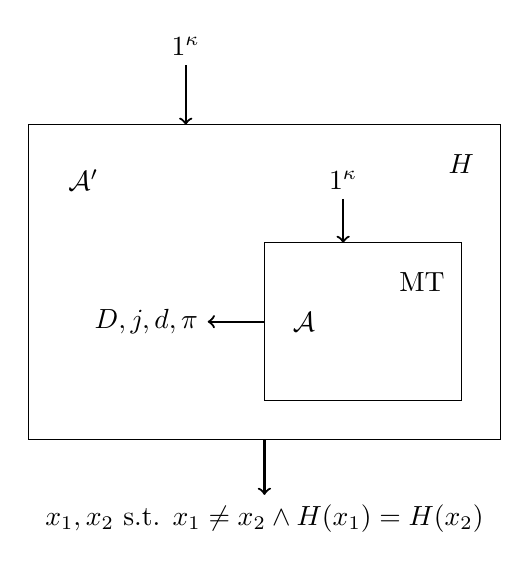
\begin{tikzpicture}
        \draw[draw=black] (0,0) rectangle (6, -4);
        \draw[draw=black] (3,-1.5) rectangle (5.5, -3.5);

        \node at (3.5,-2.5) {$\mathcal{A}$};
        \node at (5,-2) {MT};

        \node at (0.7,-0.7) {$\mathcal{A}'$};
        \node at (5.5,-0.5) {$H$};

        \node (inner_input) at (4,-0.7) {$1^\kappa$};
        \node (inner_output) at (1.5,-2.5) {$D, j, d, \pi$};

        \node (input) at (2,1) {$1^\kappa$};
        \node (output) at (3,-5) {$x_1, x_2$ s.t. $x_1 \neq x_2 \land H(x_1) = H(x_2)$};

        \draw[->, thick] (3,-2.5) -- (inner_output);
        \draw[->, thick] (inner_input) -- (4,-1.5);

        \draw[->, thick] (input) -- (2,0);
        \draw[->, thick] (3,-4) -- (output);
    \end{tikzpicture}
\end{center}

We use $e$ for the hash value calculated by the client, $h$ for the expected hash value in the correct Merkle tree, and $\pi$ for the hash values returned by the server.

Consider the event that $\mathcal{A}$ succeeds, i.e. $\mathrm{verify}(\mathrm{compress}(D), d, j, \pi) = 1 \land d \neq D[j]$.

$\mathcal{A}'$ works as follows:

Given that $\mathcal{A}$ succeeds, the returned list of $\pi$ is used to calculate hashes of the nodes to verify the returned data chunk, which involves calculating $e$ values by concatenating the children of the nodes. The hash of the root is the same ($h_\epsilon = e_{top}$)
and the hash of the data chunk is different ($e_0 \neq h_0$). (If not, $\mathcal{A}'$ has already found a collision because different data chinks have the same hash.)
Therefore, there must exist a node, some level $k$ in the tree, such that $e_k = h_k$ but its children $e_{k-1}$ or $\pi_{k-1}$ not equal to the expected $h$ values. (These must exist because roots are the same, but leaves are different). In this case, we have two different inputs that hash to the same value.

Then, adversary $\mathcal{A}'$ returns children of $e_k$ from the verifier tree at level $k$ as $x_1$ and children of $h_k$ from real tree at the corresponding position as $x_2$. Then, $x_1$ and $x_2$ satisfy $x_1 \neq x_2 \land H(x_1) = H(x_2)$.

Therefore, the probability of breaking the Merkle tree protocol is the same as the probability of breaking the collision-resistant hash function $H$.
$$
\Pr[\mathrm{MERKLE}_{\mathcal{A}}(\kappa) = 1] = \Pr[\mathrm{Collision}_{\mathcal{A}'}(\kappa) = 1]
$$

But $\Pr[\mathrm{Collision}_{\mathcal{A}'}(\kappa) = 1]$ is negligible by assumption, which means the probability of breaking Merkle tree protocol is also negligible.

\end{proof}
